\documentclass[t,12pt]{beamer}
\usepackage{helvet}
\usepackage{times}
\usepackage{courier}

\usepackage[T1]{fontenc}
\usepackage[english]{babel}

\usepackage{amssymb}
\usepackage{amsmath}
\usepackage{amsfonts}
\usepackage{graphicx}
\usepackage{color}
\usepackage{url}
\usepackage{textpos}
\usepackage{xspace}
\usepackage{array}

\graphicspath{{./fig/}}


% theme options: hy/ml/hum, rovio/sinetti, hiit
% default: hy,rovio

%\usetheme[hy]{HY}
%\usetheme[hy,sinetti]{HY}
\usetheme[hum,rovio]{HY}
%\usetheme[ml,rovio]{HY}
%\usetheme[ml,rovio,hiit]{HY}


\title[Open- and Crowd-sourced Lexicography]{Open-Source Morphologies and Crowd-Sourcing Lexicography\\\scriptsize{at FSCONS 2013}}
\author[Tommi A Pirinen]{Tommi A Pirinen \scriptsize \guilsinglleft{}tommi.pirinen@helsinki.fi\guilsinglright{} / \guilsinglleft{}flammie@gentoo.org\guilsinglright{}}
\institute[University of Helsinki]{Department of Speech Sciences\\University of Helsinki}
\date{\today}

\subject{Research}



\AtBeginSubsection[]
{
  \begin{frame}<beamer>{Outline}
    \tableofcontents[currentsection,currentsubsection]
  \end{frame}
}


\begin{document}

\selectlanguage{english}

\HyTitle
%\maketitle

\begin{frame}{Outline}
    \tableofcontents
\end{frame}

\begin{frame}{Myself and relevant projects}
    \begin{itemize}
        \item Academically: Tommi A Pirinen \url{http://www.helsinki.fi/\%7etapirine/}, see also Open science / reproducible research at \url{http://github.com/flammie/purplemonkeydishwasher}
        \item in FLOSS e.g., Flammie \url{http://dev.gentoo.org/\%7eflammie/}
        \item Open source morphology for Finnish \url{http://code.google.com/p/omorfi/}, \url{\#omorfi} on Freenode
        \item hfst-ospell \url{http://hfst.sf.net/}, \url{\#hfst}
        \item apertium machine translation, simple4all text-to-speech, 
            localisation etc. \ldots
    \end{itemize}
\end{frame}

\section{Part 1: Crowd-Sourcing and Lexical Data Concepts and Experiences}

\subsection{Introduction: Concepts}

\begin{frame}{Morphology}
    \begin{itemize}
        \item originally in linguistics: inflect words
        \item in a broad sense: classifying words, inflectional suffixes, etc.
        \item E.g., \emph{hundarnas} = hund + ar + na + s = dog, common gender,
            needs ar as plural suffix, possessive form (the dogs')
        \item \emph{Finite-State Morphology} I work with, is capable of
            much more complex language systems
        \item to reach a system dealing with this we need data about
            words, leading to...
    \end{itemize}
\end{frame}

\begin{frame}{Lexicography}
    \begin{itemize}
        \item ``Dictionary writing'', in this context more like data harvesting
        \item Collect all words
        \item How do they inflect (i.e., which are the valid forms of the word)
        \item How do they operate with other words in sentence (syntax)
        \item What do words mean, how do you translate them (semantics)
        \item Everything else
    \end{itemize}
\end{frame}

\begin{frame}[plain]{Example of trad. dictionary}
    [Oxford English Dictionary, $3^{rd}$ ed., s.v. set]
    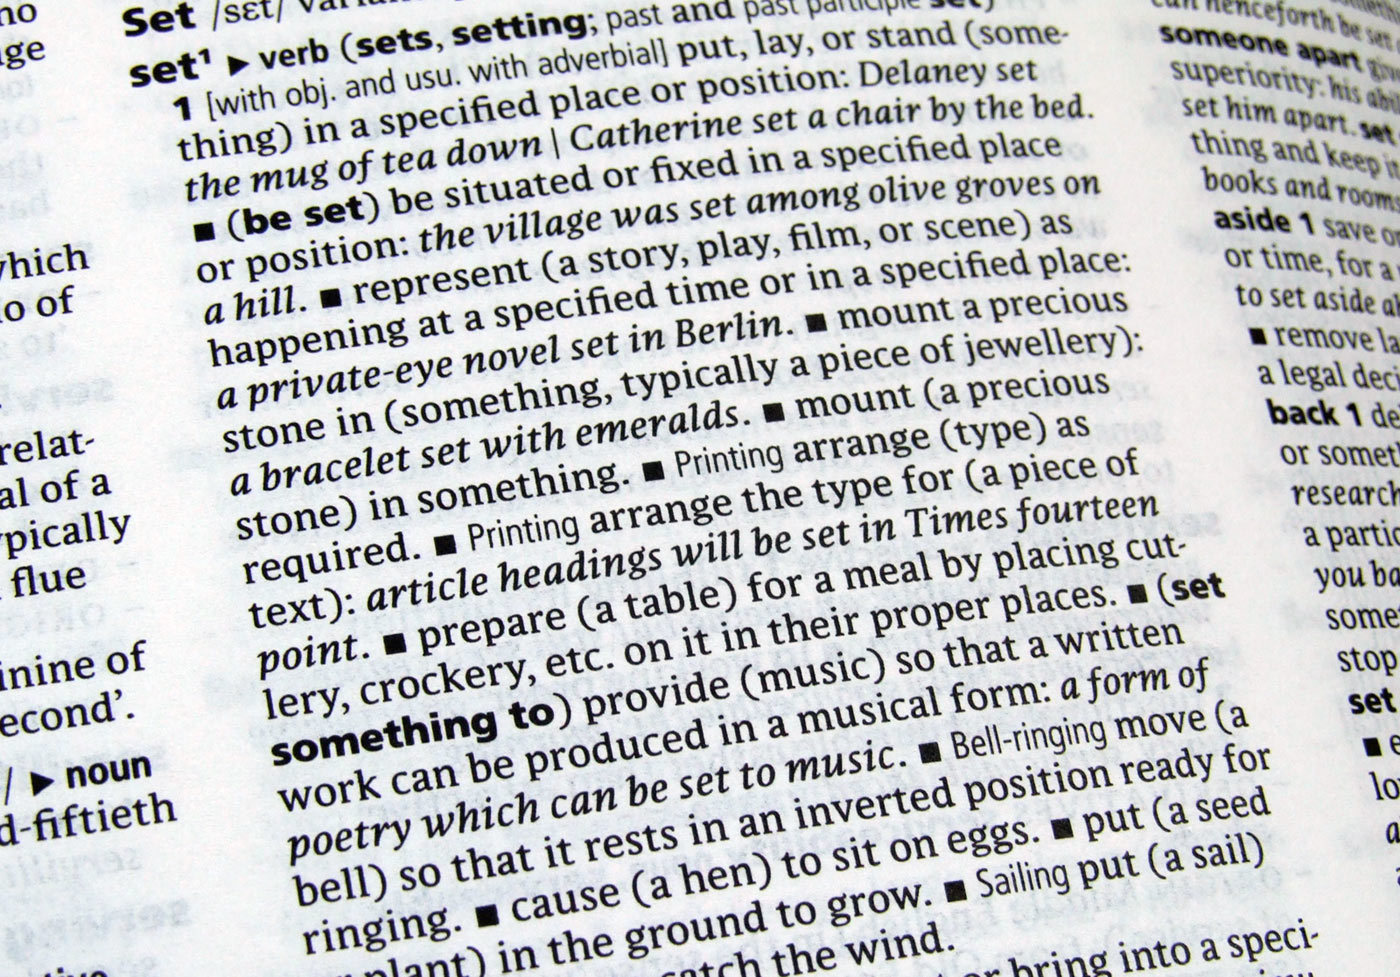
\includegraphics[keepaspectratio=true,width=1\paperwidth]{oed}
\end{frame}

\begin{frame}{One example of Digital Dictionary}
    [our Finnish omorfi database s.v. \emph{asettaa} (set)]
\texttt{
asettaa	['V\_VIEROITTAA']	VERB	53	C	False	False	None	False	False	None	aset	aset{t0}aa{\textasciicircum back}{C}	None	weaken	back	False	False	False	None	False	False	False	False	asettaa
    }
\end{frame}

\begin{frame}{Crowd-sourcing}
    \begin{itemize}
        \item Getting lots of people to work on same project
        \item Wikipedia is the best success story here
        \item Ideal for lexicography: no special skills needed, all native
            speakers know words of their language
        \item There are projects for dictionary building as well:
            Wiktionary, Omegawiki, \ldots (not as huge success stories, yet)
    \end{itemize}
\end{frame}

\subsection{Crowd-sourcing: uses and issues}

\begin{frame}{Uses of Crowd-Sourcing in Morphology Development}
    \begin{itemize}
        \item New words come and go all the time: \emph{crowd-sourcing}, 
            \emph{facebooking}, \ldots, and we need all of them ASAP
        \item Collecting new features and information bits for words never ends
        \item semantics: is it (can it be) human, sentient, edible, female,
            location, corporation, mass nouns
        \item popularity: common word, rare, obscure
        \item style and usage: dialects, curse words, academic, computer,
            medicine
        \item \ldots approx. each new application for language model needs new
            data
    \end{itemize}
\end{frame}

\begin{frame}{Issues in Crowd-Sourcing Lexicographies}
    \begin{enumerate}
        \item Using data (long) after it has been built by harvesting, scraping,
            etc. requires lots of work
        \item Inputting well-structured data in system not designed for it is
            cumber-some and error prone
        \item That is, wiktionary is really just an attempt of using something
            designed for writing encyclopedic prose in structured dictionaries
        \item Wiktionaries are never stable, trying to use data from outside
            the system requires tracking changes in conventions
        \item Newer systems attempted to bridge the gaps have not been 
            successful either (Omegawiki, ...)
    \end{enumerate}
\end{frame}

\begin{frame}[plain]{Example of Wiktionary Page}
    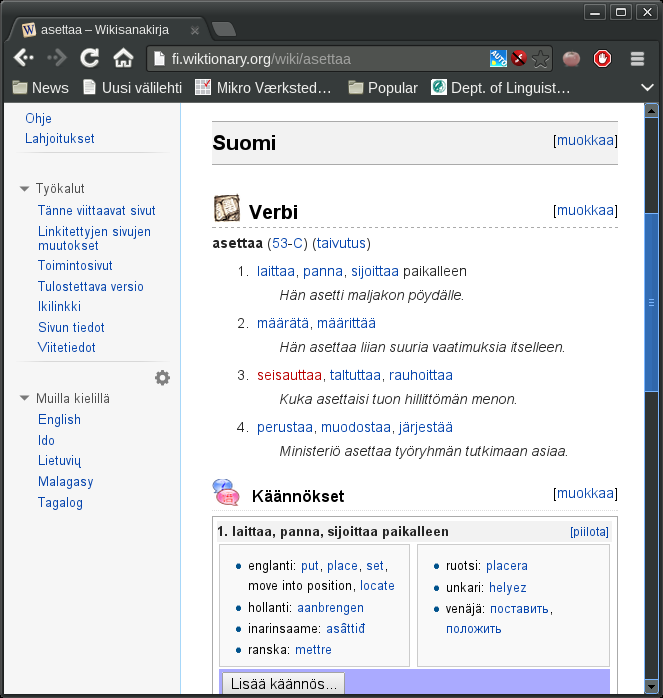
\includegraphics[keepaspectratio=true,width=1\paperwidth]{fiwikt-web}
\end{frame}

\begin{frame}[fragile]{And its Source...}
    \begin{verbatim}
===Verbi===
{{fi-verbi|as|ettaa|muistaa|C}}

# [[laittaa]], [[panna]], [[sijoittaa]] paikalleen
#:''Hän asetti maljakon pöydälle.''
# [[määrätä]], [[määrittää]]
...
====Käännökset====
{{kohta|1|laittaa, panna, sijoittaa paikalleen|
*englanti: [[put]], [[place]], [[set]], move into position, [[locate]]
*hollanti: [[aanbrengen]]
\end{verbatim}
\end{frame}

\begin{frame}{Scraping the Data From Wiktionary}
    \begin{enumerate}
        \item find section for Finnish words
        \item find each definition
        \item find and translate something like
            \texttt{fi-verbi|as|ettaa|muistaa|C}
                into \texttt{asettaa V\_MUISTAA VERB 53 C\ldots}
    \end{enumerate}
    \begin{itemize}
        \item e.g., when I last wrote the script for scraping this data,
            \texttt{fi-verbi|as|ettaa|muistaa|C} was \texttt{fi-verb|53|C}
    \end{itemize}
\end{frame}

\begin{frame}{Example 2: Omegawiki}
    \begin{itemize}
        \item database approach for storing data in well structured form
        \item getting data would be easier and more consistent
        \item still quite cumbersome to edit
        \item lacks some central pieces of infromation for Finnish and most
            other langs than English, e.g., inflection classification
    \end{itemize}
\end{frame}

\begin{frame}[plain]{Example of Omegawiki Page}
    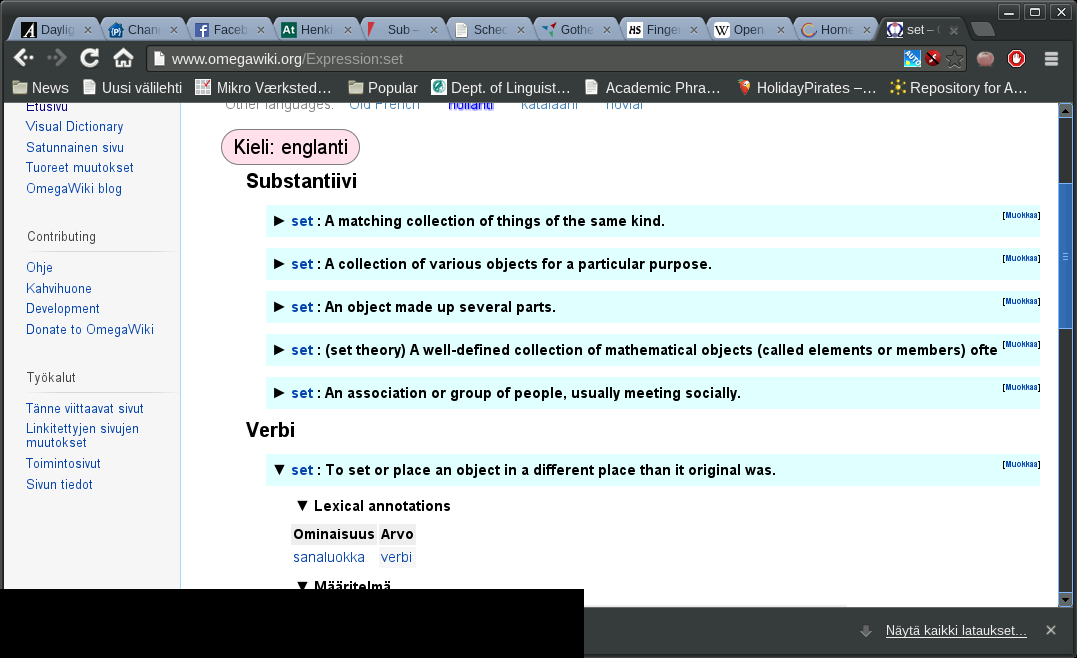
\includegraphics[keepaspectratio=true,width=1\paperwidth]{omegawiki}
\end{frame}

\begin{frame}{Quality Issues in Crowd-Sourcing}
    \begin{itemize}
        \item people know lots of their native languages but not always enough
        \item some contributors are language learners
        \item vandalism
        \item Two ways currently used to cope with this: python scripts, regexes
            etc. to check some sanity
        \item Automatic tests with the final software and free texts: do new
            additions work somewhat like old words, etc.
        \item In the end it all falls down to expert reviews again
    \end{itemize}
\end{frame}

\begin{frame}{Conclusions (questions): How to Proceed?}
    \begin{itemize}
        \item How to combine popularity of Wiktionary with forms and structure
            of Omegawiki?
        \item Improve user interfaces?
        \item Better access to wiki data?
        \item Feedback from databases to Wiktionary?
        \item Answers? Questions? 
    \end{itemize}
\end{frame}

\HyTitle

\section{Part 2: Productising Research Results}

\begin{frame}{Myself and relevant projects (again)}
    \begin{itemize}
        \item Academically: Tommi A Pirinen \url{http://www.helsinki.fi/\%7etapirine/}, see also Open science / reproducible research at \url{http://github.com/flammie/purplemonkeydishwasher}
        \item in FLOSS e.g., Flammie \url{http://dev.gentoo.org/\%7eflammie/}
        \item Open source morphology for Finnish \url{http://code.google.com/p/omorfi/}, \url{\#omorfi} on Freenode
        \item hfst-ospell \url{http://hfst.sf.net/}, \url{\#hfst}
        \item apertium machine translation, simple4all text-to-speech, 
            localisation etc. \ldots
    \end{itemize}
\end{frame}

\subsection{Introduction}

\begin{frame}{Case of Creating Spell-Checkers for Less-Resourced Languages}
    \begin{itemize}
        \item Research work: Moving from open source morphologies to efficient
            finite-state spell-checkers
        \item Including conversion from existing formats to something equivalent
            of finite-state automata (e.g., from hunspell and its predecessors)
        \item At the moment: Software exists, is usable in enchant, libreoffice,
            etc., but not available in distros
    \end{itemize}
\end{frame}

\begin{frame}{Current Research Methodology}
    \begin{enumerate}
        \item Research problem (issues in current spell-checking)
        \item Idea for solution (scribbled notes and formulas)
        \item Proof-of-concept implementation (hacky code)
        \item Experimentation (one-off measurements)
        \item Publication
        \item ... Research projects, funding etc. end here, all results get abandoned
    \end{enumerate}
    Results, data, code, is all published in open science terms.
\end{frame}

\begin{frame}{Suggested Continuation}
    \begin{enumerate}
        \item ... Publication 
        \item Software Development (from hacky code to real library)
        \item Integration to Real World Software
        \item Distribution
        \item Maintenance
        \item Profit
    \end{enumerate}
\end{frame}

\subsection{Some examples}

\begin{frame}{Example from Early Part of my Project}
    hunspell2fst, would be rather important in business of replacing hunspell:
    \begin{enumerate}
        \item Transforming existing hunspell dictionaries into more efficient
            finite-state spell-checkers
        \item Few obscure formulas: ....
        \item Then some flex and yacc code and scripts
            to transform hunspell data files in around 10 commands
        \item Measured some improvement over hunspell on most of the languages
        \item Published in 2010 in an IEEE journal
        \item The collection of scripts used is probably unusable now
    \end{enumerate}
\end{frame}


\begin{frame}{Compare to: End of my Thesis Project}
    \begin{itemize}
        \item Full working spell-checking, faster than hunspell, more efficient
            in most cases (but likely less stable)
        \item Integration to common open source software: LibreOffice,
            Mozilla, enchant (GTK+) (via software library voikko)
        \item Standard installation but turned off by default, requires manual
            work and not in current distributions, but packages exist
    \end{itemize}
\end{frame}

\subsection{Requirements for a Software Product}

\begin{frame}{Product Requirements Unmet by Typical Scientific Software}
    \begin{itemize}
        \item Stability: no error checking, no crash guarding, ... since software
            is only used in protected env. by experts without malicious intents
        \item Licencing: Academic licence restrictions are strictly against
            GNU definition of Freedom; smaller discrepancies, e.g., Debian legal
            does not allow even GPLv2 and Apache2 on same software
        \item Standards: GNU standards, not only for licence but installation
            procedures, packaging
        \item User interfaces: GNU, Gnome, KDE, ... integration
        \item Documentation: Academic paper is not code documentation or so 
            forth 
    \end{itemize}
\end{frame}

\begin{frame}{Other Issues}
    \begin{itemize}
        \item Software maintenance in Linux distributions requires committed
            people to work on it (e.g., I only have access to gentoo's web since
            lack of activity etc.)
        \item Getting access to Linux distribution systems requires social
            engineering
        \item Niche products (limited use scientific software, small
            languages' support) may be frowned upon by software engineers. E.g.:
        \item ``Well, that's a valid enhancement request, of course, but something must to be done to prevent filling the text language dropdown with \alert{such rubbish languages}, making it hard to use.'' a comment to bug report asking for Kumyk
            support in LibreOffice
    \end{itemize}
\end{frame}

\begin{frame}{Windows Support? And other systems; Android, Mac OS X?}
    \begin{itemize}
        \item Windows support usually requires commercial contracts, non-free
            implementations, NDAs
        \item For spell-checking, Windows 8, Android 4, Mac OS X are gradually
            opening the access to spell-checking components that can be used
            to replace or extend system libraries
        \item In general, software product maintenance could be passed over
            from scientist to hobbyists and commercial workers, 
    \end{itemize}
\end{frame}

\begin{frame}{Conclusion: Questions? Answers?}
    \begin{itemize}
        \item Open science and FLOSS is not enough for all (any?) academic
            projects to become products (in FLOSS envs even)
        \item Scientists are scarce resource for software development,
            maintenance, distribution...
        \item
    \end{itemize}
\end{frame}

\begin{frame}{Links and References}
    \begin{itemize}
        \item foo
    \end{itemize}
\end{frame}

\end{document}
% vim: set spell:
